\documentclass[oribibl]{llncs2e/llncs}
\usepackage{geometry}                % See geometry.pdf to learn the layout options. There are lots.
\geometry{letterpaper}                   % ... or a4paper or a5paper or ... 
%\geometry{landscape}                % Activate for for rotated page geometry
%\usepackage[parfill]{parskip}    % Activate to begin paragraphs with an empty line rather than an indent
\usepackage{amssymb,amsmath}
\usepackage{graphicx}
\usepackage{amssymb}
\usepackage{epstopdf}
\DeclareGraphicsRule{.tif}{png}{.png}{`convert #1 `dirname #1`/`basename #1 .tif`.png}

\graphicspath{{WarpTask/figures/}{Res/figures/}} %do not forget the / at the end
%\include{{llncs2e}}
\title{Very Large Integers  and polynomial inner products}
\author{Timoth\'ee Ewart\inst{1}\thanks{Acknowledgments: Maxim Milakov, Peter Messmer:   NVIDIA,   Williams Sawyer, Gilles Fourestey:  CSCS, HP2C funding, hp2c.ch}  , Andreas Hehn$^2$, Matthias Troyer\inst{2} and Thierry Giamarchi\inst{1}}

\institute{Universit\'e de Gen\`eve, \email{timothee.ewart@gmail.com}  \and Eidgen\"ossische Technische Hochschule Z\"urich }

%\date{}                                           % Activate to display a given date or no dater
\begin{document}
\maketitle
%\section{}
%\subsection{}
%\vspace{-0.65cm}
\begin{abstract}
The main purpose of the  Very Large Integer (VLI/C++/ASM) library is to perform large integer arithmetic and  inner products of polynomials. Based on meta-programming of assembly language,
and  hybrid (CPU/GPU) mode, it performs inner products of dense and triangular polynomials  of 1 to 4 variables  where the coefficients are represented  by large integers of 128 to 512 bits. 
In this paper, we present the basics of the inner products of polynomials, and  the implementation of the library for the CPU and the GPU.  All our algorithms are based on brute force attacks, because the problem is too small for a FFT approach. We save a factor up to 10 on CPU, and 60 on GPU compared to a GMP solution,
and attain 67 \% of the peak performance of the GPU.
\end{abstract}
\section{Introduction}
% TODO references LINBOX, NTL

The Very Large Integer library performs  standards  operations for large integer arithmetic and polynomial. This library also provides optimized implementations of inner products  for GPU.
This library is composed of two distinct modules,  but enough closed  to work together by the mechanism of template instantiation. VLI is a fix size library from 128 to 512 bits,
as the polynomial module  which is limited for dense and triangular polynomials  up to 4 variables. The core of VLI is build under ASM language to provide the best performance.  Every arithmetic operations
are executed by a specific kernel generated specifically during the compilation by an ASM generator. Moreover, VLI allows multithreading and hybrid  GPU usage for inner products of polynomials.
Multithreading is build on OpenMP library and GPU module under CUDA. As the CPU, the GPU is a fixe size library, and ASM kernels are also determinated specifically during the compilation.

In large arithmetic, the standard library is GMP\footnote{GMP is the standard library for long arithmetic, gmplib.org}. GMP is polyvalent, nevertheless this polyvalence is attained by the usage of  dynamic memory.
It is well know dynamic allocation is time consuming, and it can become a bottle neck for small operations which are in the working range.  
Alternatively for polynomial arithmetic, a few libraries like  LINBOX or NTL  provide a solution but  they use GMP when needed. 
Although hardware accelerators were introduced  in HPC a few years ago, as the GPUs  by NVIDIA. Only a few libraries have been adapted 
A prominent example of such an adaption are the MAGMA libraries, which port the well known BLAS/LAPACK packages to GPU accelerators.
The polynomials libraries, however,  have not done the transition to these new hardwares yet.
During the last few years, the polynomial multiplication was successfully implemented on this new hardware
\cite{Govindaraju2008, Emeliyanenko:2009, Moreno2010}. All these works focus on large polynomials, using a FFT approach. 

In this work, we are going to highlight the speedup given by a tiny ASM library without any dynamic memory, suggest an alternative for small size integer. 
And propose an efficient implementation of inner product on GPU with the latest CUDA PTX features.  

%In the present work, we focus on the inner products of dense and triangular multivariable polynomials.  The coefficients of the polynomials are large integers. 
%In contrast to GMP which dynamically adapts the size of the integers, the presented long integer library is based on static integer sizes.
%Moreover, our library is natively compatible with GPU to allow hybrid calculation. GPUs impose contiguous memory which is impossible with a GMP approach due to the dynamic allocated memory.
%Thus, we propose a  library based on contiguous memory where the exact assembly kernels are generated during the compilation for CPU and GPU.
%The static integer sizes allow the compiler to aggressivly optimize the non-assembly parts of the library and avoids costly heap allocations for the data. 

\section{Polynomial and inner products definitions}

The library performs standards operations for polynomials (up to four variables) and optimized solvers for  the inner products of vectors of polynomials (presented in the next section).
The polynomials are defined like  e.g. our variables
\begin{eqnarray}
P_a(x,y,z,w) & = & \sum_{i=0}^n \sum_{j=0}^n  \sum_{k=0}^n \sum_{l=0}^n  a_{ijkl} x^i y^j z^k w^l , \,\,\,\,\,\, \text{or} \\
                   & = & \sum_{i=0}^n \sum_{j=0}^{(n-i)} \sum_{k=0}^{(n-i-j)} \sum_{l=0}^{(n-i-j-k)}  a_{ijkl} x^i y^j z^k w^l  .
\end{eqnarray}
where  $x,\,y,\,z$ and $w$ are symbolic variables,  $i,\,j,\,k$ and $l$  the indices, $a$  the coefficients, and $n$ the order of the polynomial.
The polynomials of the form  (1) and (2) are named dense and triangular respectively. Consider now two vectors of polynomials of the  same type with $m$ 
entries  $\boldsymbol{v}_1$ and  $\boldsymbol{v}_2$. The inner products  consist of the product 
of all entries  associated with a global reduction. 
 \begin{eqnarray}
 P_c = \sum_{i=0}^m \boldsymbol{v}_{1_i} \times  \boldsymbol{v}_{2_i}  \label{poly1} \label{InnerProduct}
\end{eqnarray}
where $\times$ indicates the multiplication between two polynomials. The multiplications use usual rules of polynomials multiplication. 
A final coefficient may be the sum of several coefficients (which we call contributions in the following passage), resulting from the sum of several multiplications. These coefficients are the cross terms. 
The cross terms are not a problem for the CPU version, as a polynomial multiplication is done by a single thread, but they are the bottleneck for the GPU version.
The number of coefficient for a dense and triangular polynomial is given by $(n+1)^{\kappa}$ and  $(\kappa+n-1)! / ( (\kappa-1)! n! )$ respectively, where $\kappa$ is the number of variables. 

In terms of  programming and parallelization, in the CPU version, the previous equations can be reduced to independent loops with a final reduction.
The CPU parallelization has been done with OpenMP. The OpenMP threads calculate several  polynomial multiplications and make a local reduction. At the end, a final reduction is performed  by the main thread.
 % \footnote{In OpenMP reduction for class is not supported}. Results showed a perfect scalability of the OpenMP code. 

\section{VLI  CPU library}

The coefficients of the polynomials are represented by a large integer named the VLI number.  A VLI number is characterized by a size in bits.
Our current implementation allows for integer sizes from 128 to 512 bits, but is easily extendable to larger integers.
Inside the memory, the VLI numbers are  contiguous. The data type container is a 64 bit unsigned integer array.

The basic operations supported by VLI are the four basic operations: $+,-,\times, /$, extended multiplications and bit shift. The library allows  operations between operands of the same type, and with basic  integers. 
For performance reasons, we have a specific solver for every operation except  for division.
All the algorithms and operations are based on basic arithmetic but have been implemented in assembly language to make use of hardware features which are not accessible by plain C++.

\subsection{Assembly language}

We applied algorithms based on childhood  experience for large arithmetic. The implementation necessitates a carry bit and an extended multiplication. The hardware supports
the carry bit in the status register, as the extended multiplications, but they are only accessible by the assembly language.
In assembly, these operations  are supported by the pair of mnemonics; \texttt{addq/adcq} for the addition; \texttt{subq/sbbq} for the subtraction, and \texttt{mul} for the extended multiplication.   
Combining these mnemonics, we reproduce easily long arithmetic algorithm, as described into the famous  ASM book of \cite{Hyde:2003:AAL:861534}. 

We coded the kernels using the GNU inline assembly.
Generating by hand all these  assembly strings (kernels)  can be painful and error-prone\footnote{The library has near 10000 lines of assembly in total for x86-64, Power64, and PTX}.
We designed a assembly generator. It creates all versions of a kernel during the compilation.   
It is built on Boost preprocessor package. We can thus create and manipulate the ASM strings during the compilation, 
and generate a specifically tuned kernel for every large integer. We give a small example of a long addition with the generator into the table \ref{ASMGENERATOR}.

 \begin{table}[h] 
	\begin{center}
	 	\begin{tabular}{l l}
                           \hline 
                           \textbf{Assembly generator}      \hspace{8.5 cm}  ASM  x86-64 \\ \hline
                           \begin{tabular}{l l l l } 
                               \tiny{1:} &  asm(\texttt{"}     &  $\vartriangleright$ Start ASM string & asm(\texttt{"} \\
                               \tiny{2:} &  \textbf{boost  repeat} over n  &$\vartriangleright$  Start the repetition over n from 0 to n-1 &   \\
                               \tiny{3:} &   \hspace{0.2 cm}  boost  if(n = 0) &  $\vartriangleright$   if n = 0 &  \hspace{0.2 cm}  \texttt{"}\texttt{addq} 0x0(rsi), rax\texttt{"}\\    
                               \tiny{4:} &   \hspace{0.4 cm}  boost stringize(\texttt{addq}  $r_i$, $r_j$)  &$\vartriangleright$   Become \texttt{"addq} \dots &  \hspace{0.2 cm}    \texttt{"}\texttt{adcq}  0x8(rsi), rax\texttt{"}\\    
                               \tiny{5:} &   \hspace{0.2 cm}  boost  else  & $\vartriangleright$   if n != 0 &  \hspace{0.2 cm}  \texttt{"}\texttt{adcq}  0x10(rsi), rax\texttt{"} \\ 
                               \tiny{6:} &   \hspace{0.4 cm}  boost stringize(\texttt{adcq}  $r_i$, $r_j$)  &$\vartriangleright$   Become \texttt{"adcq} \dots &  \hspace{0.2 cm}   \texttt{"}\texttt{adcq}  0x18(rsi), rax\texttt{"}\\     
                               \tiny{7:} &  \textbf{end boost repeat} &  &   \\                            
                               \tiny{8:} &  \texttt{"})  &  $\vartriangleright$ end ASM string & \texttt{"})\\
                          \end{tabular} &  \\ \hline
		 \end{tabular} 
		 \caption{Simplified  example of the ASM generator for a long addition (n=4), the Boost preprocessor macros generate the effective string for the ASM block. ASM \texttt{move} are not included. \label{ASMGENERATOR}  }
	\end{center}
\end{table} 

The x86-64 architecture allows 16 registers (32 for Power architecture). We try to reuse the data in the registers as much as possible in order to reduce memory read/writes to the minimum.  Additional optimizations have been done like full unrolling and assembly tips. We  supported  x86-64, Power64 and PTX (GPU) assembly language.
 PTX does not support carry bit for 64-bit integers, but only for 32-bit integers\footnote{Introduced since CUDA 4.2}.  
It allows a fused multiplication-addition of 32-bit integer  with carry bit support \cite{CUDAasm}. 
The calculation in 32-bit mode imposes twice as much operations for the additions/subtractions, and one order of magnitude more for the multiplications. 

\subsection{Memory layout and SIMD possibility}

We have privileged the  array  of structure  (SoA ) detrimental to the  structure of array (SoA)
The AoS consists in saving the data in this hierarchy: VLI - series of VLI (polynomial coefficient) - series of polynomials (the vector), where  the SoA structure interleaves the coefficients of the VLI and the polynomials.
A representation of both memory layout is presented on figure \ref{AOSSOA}. 

\begin{figure}
    \begin{minipage}{0.50\linewidth}
        \begin{eqnarray}
        \tiny{
                 \underbrace{
                 \underbrace{ \underbrace{a^0_{00} | a^1_{00} | a^2_{00}}_{VLI, a_{00} } || \underbrace{a^0_{10} | a^1_{10} | a^2_{10}}_{VLI, a_{10}} ||   \dots  }_{1^{st} \textrm{polynomial}} 
                  |||    \underbrace{ \underbrace{b^0_{00} | a^1_{00} | b^2_{00}}_{VLI, b_{00} } || \underbrace{b^0_{10} | b^1_{10} | b^2_{10}}_{VLI, b_{10}} ||   \dots  }_{2^{nd} \textrm{polynomial} } }_{\textrm{Vector of polynomials, AoS order}} \nonumber
            }
        \end{eqnarray}
    \end{minipage}
\begin{minipage}{0.50\linewidth}
    \begin{eqnarray}
    \tiny{
        \underbrace{
        \underbrace{a^0_{00} | a^0_{10} | \dots || a^1_{00} | a^1_{10} | \dots  }_{1st  \textrm{ nested VLI/Polynomial} } |||  \underbrace{b^0_{00} | b^0_{10} | \dots || b^1_{00} | b^1_{10} | \dots  }_{2nd  \textrm{ nested VLI/Polynomial} }
        }_{\textrm{Vector of polynomials, SoA Order}} \nonumber }
        \end{eqnarray}
\end{minipage}
\caption{Representation of the AoS Order (left) or SoA Order (right) for a vector of polynomial \label{AOSSOA}.  The SoA structure limits the usage of the VLI module alone.}
\end{figure}

We have choose the SoA for the two following reasons :

\begin{enumerate}
\item SoA order allows the natural propagation of the carry bit between the entries of the VLI with the pair of mnemonics \texttt{addq/adcq}, as the utilization of the extended multiplication without any padding.  
\item The VLI and the polynomial module of the library can be separated and use independently. Thinks impossible if the coefficients are interleaved.
\end{enumerate}

The disagreement  of this choice, the SoA order does not facilitate the usage of the SIMD instruction such as the AVX instructions of the Sandy Bridge x86-64 architecture.
Applying SIMD to the AoS, for an addition or a subtraction is a nonsense because there is no specific instruction to propagate carry bit between entries of the SIMD register.
It could be  apply  on multiplications for integer  larger than 1024-bit \cite{SIMD}, unfortunately, it does not correspond to our working range. Consequently, we do not 
use the multimedia instruction into the ASM kernels.

%The choice of the memory layout is important. It may facilitate  the usage of the SIMD instructions such as the AVX instructions of the Sandy Bridge x86-64 architecture. We choose the AoS for the following reasons:
%Applying SIMD to the AoS, for an addition is a nonsense because there is no specific instruction to propagate carry bit between entries of the SIMD register.
%The extended multiplication under AVX \texttt{\_\_mm256\_mul\_epu32}  allows only four multiplications of 32-bit, saving a factor of two, nevertheless, on Sandy Bridge, we have 3 ALU, we can not exclude
%the execution of several long multiplication at the same time, and we lose the benefit of the SIMD version. Moreover, there is a large overhead  to prepare the registers and shuffle the data into the registers. For our range of operations the extended multiplication varies from 128 to 512 bits, a SIMD version will not be the optimal solution. However SIMD has been used with success for  integers larger  than 1024-bit \cite{SIMD}.
% TODO somehow the problem with SIMD operations is not entirely clear yet. You mention the issues, but I think you should elaborate them a little more.

%\section{A short introduction to GPU}

%A Graphical Processing Unit  is efficient  to address problems which can be expressed as data-parallel computations, where the same stream of instructions
%is executed on many data elements in parallel. Successful usage of GPU in HPC requires a good understanding of their design to reach great performance. A GPU is composed 
%of several independent calculation  entities named streaming multiprocessors (SMs typically 4 to 12), where the SMs run hundreds of threads concurrently (typically 256) in groups of 32 threads (called ``warps'').
%The GPU programming model divides the problem into coarse sub-problem that can be solved independently in parallel by blocks of threads,
% and each sub-problem into finer pieces that can be solved cooperatively in parallel by all threads within the block.

%In terms of memory, all SMs  share  a large  memory (several GigaBytes) with  low performance but  high performance compared to CPU main memory; approximatively one hundred cycles for read/write operations. Inside each SM additional special memories (constant, shared, texture, surface) are available. These memories are characterized by their behavior: they can be read only, shared, cache and more.   They still have common characteristic: a very high performance for read/write  operations in a few cycles only.
%A good programming practice is to preload data from global memory in shared/texture at once, for subsequent computations.  \label{CUDA_PRACTICE}

%Applying the GPU ideology to the polynomial inner products  means that the polynomial multiplications will be executed in parallel on the SMs. Then a global reduction will sum all resulting polynomials. The division into blocks is natural, a block being a single entry of the vector (equation \ref{InnerProduct}).  The difficulty consists of designing a parallel algorithm for the polynomial multiplication and the final reduction.

\section{Inner product booster on GPU}

%The first idea comes to mind: calculate every single multiplication on an independent GPU thread. Indeed for a dense polynomial, the number of coefficients can be large and compatible with the number of SMs threads. Nevertheless, the resulting coefficients may have several contributions. If the contributions are calculated by several threads, this requires reduction between threads. This solution introduces   synchronizations and leads to low performance.

The GPU algorithm of the inner product is divided into two parts. A preliminary step on the CPU,  where we prepare the calculation blue print of the  contribution. And the calculation itself on the GPU

\begin{enumerate}

\item  First, we create a dummy resulting polynomial  represented by the indices and the contributions. They are sorted by descending order of the number of contributions
and grouped by 32 as a task.   A task is a set of 32 resulting coefficients in a specific order. It tells a  warp how to calculate coefficients (the thread number one of the warp takes the first coefficient of the task and so on).
These tasks are reordered over the warps to balance the amount of work. An illustration of this algorithm is given on  figure \ref{algo_GPU}. 
The more coefficients the polynomials have, the more uniform the distribution of the tasks over the warps will be, and the more efficient the calculation.
We fix the maximum number of warps to eight (8 warps/256 threads), as far as possible, we assign at least two tasks per warp.
Thus, depending on  the number of coefficients a warp may calculate one task, whereas another warp may have several tasks to calculate.
When the determination of the list of the tasks is over,  we transfer  asynchronously  to the global memory the data of the polynomial and all the tasks.
This method does not  change the ordering of the data, ss for the CPU version, we have an AoS order.
But we have now informations how calculate the polynomial into a efficient way.
In terms of memory of the GPU, we allocate allocated only once, and reuse inner products after inner products., thus we save time.

\begin{figure}[t]
\begin{center}
\mbox{
\includegraphics[scale=0.37, angle=-90]{coeffs.eps} 
\includegraphics[scale=0.37, angle=-90]{warp.eps} 
}
\caption{Left: Results coefficients (red line) sorted in reverse order and group by warp. Right: Balance of the tasks over the warps.}
\label{algo_GPU}
\end{center}
\end{figure}

\item  Second, at the beginning we  cached both input polynomials into the texture memory. 
When a polynomial multiplication begins,  every warp gets the corresponding tasks (at least one) from the task's list and loops over its number of tasks. Then,
the threads in a warp get their respective output coefficients and iterate over the number of  contributions.
For every iteration over contributions, the threads determine the input coefficients, read the corresponding data in the texture memory, and perform the arithmetic operations: an extended multiplication and an optional long addition (if the result coefficient has several contributions). The calculation of an output coefficient  is  done in fast memory (texture for the input data, and register for the intermediate result). 
When the loop over contributions terminates,  we transfer the coefficients into the an intermediate buffer in the global memory, but in SoA  order for the final reduction. 
The reduction is done using the standard method of NVIDIA \cite{CUDAReduction} to achieve the highest performance.

 \begin{table}[t] 
	\begin{center}
	 	\begin{tabular}{l l}
                           \hline 
                           \textbf{Task execution}  Algorithm &  \\ \hline
                           \begin{tabular}{c l l} 
                               \tiny{1:} & VLI tmp   &  $\vartriangleright$ Specific to every thread  \\
                               \tiny{2:} &  \textbf{for} over number of task list size &$\vartriangleright$  Depend on the warp \\
                               \tiny{3:} &   VLI ResCoeff &$\vartriangleright$  Thread gets a result coefficient from a task \\
                               \tiny{4:} &  \hspace{0.2 cm}  \textbf{for} over the number of contributions  & $\vartriangleright$ Each thread loops over its coefficients \\
                               \tiny{5:} &  \hspace{0.4 cm}   Indices$_i$ = GetIndices(ResCoeff) &$\vartriangleright$ Determine input indices \\
                               \tiny{6:} &  \hspace{0.4 cm}   tmp + = CoeffPoly$_1$(indices$_1$) $\times$ CoeffPoly$_2$(indices$_2$) &$\vartriangleright$ Perform the extended MulAdd  \\
                               \tiny{7:} &  \hspace{0.2 cm}   \textbf{end for} &\\
                               \tiny{8:} &  SaveSoA(tmp) & $\vartriangleright$ Write into the global memory under AoS \\                               
                               \tiny{9:} &  \textbf{end for} &\\                               
                          \end{tabular} &  \\ \hline
		 \end{tabular} 
		 \caption{Algorithm of the task execution on GPU for the polynomial multiplications. \label{ALGO}}
	\end{center}
\end{table} 


\end{enumerate}


This algorithm gives good  performance on a GPU because the warps have approximatively the same amount of work,  and every thread in a warp will be responsible for all contributions to an output coefficient.
The contributions are not dispatched between the threads, thus we do not  introduces   synchronizations and leads to low performance. 
This  algorithm has the great advantage of working well with dense - triangular polynomials, and it could be extended to sparse polynomials, as structure of the polynomial is not primordial.
The main difficulty consists  of designing an efficient function GetIndices (\ref{ALGO}) which determines the contributions.

To conclude,  We also developed an optional hybrid mode between CPU/GPU. This  technique is usual in GPU computing.
We split the input vectors of polynomials into two chunks of data, execute concurrently on CPU and GPU. 
A synchronization  is performed during  the memory transfer   by the final reduction, at the end of the calculation.

\section{Results}



Benchmarks are performed on the facilities of the Swiss Center for Scientific Computing (CSCS), on a Cray  XK7 cluster for the GPU, and a Sandy Bridge  node with 32 logical cores  (HyperThreading on) Xeon E5-2670. The size of our vector is equal to 4096, the order of the polynomials varies from 1 to 14, the size of the input coefficients of the polynomials varies from 128 to 256 bits, the output polynomial has double width-coefficients (256 to 512 bits). 

We compute the  result  numbers as operations \footnote{An operation can be a long multiplication, addition and so on}   per seconds $GOP/s=10^{-9} \times batch/t$, where  $batch$ is the number of long integer operations computed during the execution (additions and multiplications), $t$ [s]  is the elapsed time. For more realistic comparison the execution time for GPU contains the memory  transfer. Contrary to Floating-point, we can not present Integers operations as FLOPS, in fact nteger operations are performed by ALU (and not on the FPU),  the number of  ALUs  between processors (Intel, AMD, IBM) and the execution time of the operations are  not constant \cite{ASMcost} (quasi - constant for FPU). We could calculate a MIPS (Million Integer Per Seconds) by counting all the integer instruction into our code and divide by the elapse time. But, we can not compare to any peak of performance, because the integer peak is really different from addition to multiplication, as well show by \cite{Vladimirov2012}. 

Figure \ref{ResME} presents the performance of a dense and triangular polynomials inner products. It compares our CPU library to GMP (where polynomials are  instantiated with VLI or GMP). We get an excellent speed-up factor from 4 to 11, for three reasons.
Coefficients of the  polynomial are allocated in one large block on the heap, while in the case of GMP, each coefficient needs to be allocated independently. It is well known that better performances are obtained with less dynamic memory allocations. The second reason is that  the meta-programming allows the construction of a specific solver for every type of large integer during the compilation, thus, we do not have a universal solver, the solver being unique with the maximum optimizations. Thirdly, the datas stay in the registers during an arithmetic operation.
  
The GPU curves show again an excellent speed up  factor of 10 to 60 maximum, compared to GMP, but with an interesting feature. 
For both kinds of polynomials, the performance for one variable is low, because we have a small number of threads during the execution of the GPU algorithms.
As the number of threads is fixed by the number of coefficients, $2n$ for a dense polynomial,  the maximum number of threads will be 28
 which corresponds to one warp. We do not utilize the full capacity of the GPU. For two and more variables, whatever the polynomials, 
  we attain the maximum performance,  if the following conditions are satisfied: The number of running threads is maximum (256 threads), and both input
  polynomials  are cached into the texture memory. On Kepler the size of the texture memory is equal to 48 kB. This memory  is highly optimized for repetitive and random access in contrast to shared memory
 where bank memory conflicts may appear. Moreover, for high orders the resulting polynomials have more coefficients which eases the the work balance between different threads and consequently improves efficiency.
 
\begin{figure}[t!]
\begin{center}
\mbox{
\hspace{-0.5cm}
\includegraphics[scale=0.37, angle=-90]{ME128.eps} 
\hspace{-0.4cm}
\includegraphics[scale=0.37, angle=-90]{MC128.eps} 
%\hspace{-0.4cm}
%\includegraphics[scale=0.25, angle=-90]{ME256.eps} 
}
\caption{Left: Inner product of dense polynomials with up to 3 variables and 126 to 256 bits coefficients. Right: Inner product of triangular polynomials with up to 3 variables and 126 to 256 bits coefficients.  Size of the vector 4096. For four variables we are limited by the memory of the node. GMP gives similar results whatever the polynomials.}
\label{ResME}
\end{center}
\end{figure}

\begin{figure}[t!]
\begin{center}
\mbox{
\hspace{-0.5cm}
\includegraphics[scale=0.37, angle=-90]{ME128MIPS.eps} 
\hspace{-0.4cm}
\includegraphics[scale=0.37, angle=-90]{MC128MIPS.eps} 
%\hspace{-0.4cm}
%\includegraphics[scale=0.25, angle=-90]{ME256.eps} 
}
\caption{Inner products of  dense and triangular polynomial   in [GIPS]. From 1 to 4 variables with 128 to 256 bits coefficients. Size of the vector 4096.}
\label{ResMEMIPS}
\end{center}
\end{figure}  

For the small orders the number of GPU threads is lower than 256 but it will increase with the order until the maximum.
After that, for the large orders the polynomials will be too large to be cached by texture memory properly. So the execution kernel calls data from the global memory which reduces the performance.
 All this behavior shows the differences between a CPU and a GPU. A CPU has  more transistors for the  data caching and flow control, it ensures a regular and optimal access to the data. For the GPU,
 the programmer manages the flow control by hand. In return, it will have more transistors for the data processing, and consequently more performance.

Although translating the results into MIPS is difficult, we attempt it, at least on the GPU, because the GPU kernel of the extended multiplication utilizes only one PTX instruction (\texttt{madc}), we can compare to a theoretical peak.
 Counting the total number of  this ASM instructions during  the inner products, and dividing by the elapsed time, we obtain an estimation in GIPS (Giga Instructions Per Second). A  profiling of the code with the CUDA profiler indicates that the bottleneck of the application is the product of polynomials, so we do not take into account   the transfer of the data and the ASM belonging  to the reduction. Therefore, we underestimate the performance of the library.
The peak performance of  a sample card based on Kepler GK110 is evaluated easily from CUDA documentation: for 32-bit integer multiply-add on 14 SMs * 700 MHz * 32 instructions per clock per SM = 314 GIPS. The results are reported in the figure \ref{ResMEMIPS}. We obtain 67\% of the peak performance of the Kepler card, which is a good result. The results are better for the dense polynomials because the function \texttt{GetIndices}  of the GPU algorithms is more time consuming for the triangular polynomials.

\section{Conclusions and future work}

The VLI library provides efficient solvers for the 128 to 512 bits integer associated with polynomials of 1 to 4 variables. We obtain a comfortable speed up as high as  60 compared 
to GMP for a specific range. The limited performances of GMP for small size were the main argument to develop the VLI library, although GMP excels in thousand bits arithmetic where our library can not operate. 
As future work, we would like to implement, new kinds of polynomials, and a better management  of  the memory to maintain the performance on GPU. And them, we would like explore new  SIMD architecture Xeon PHI where the carry bit is implemented.

\bibliographystyle{llncs2e/splncs}
\bibliography{biblio/vlibib}


\end{document}  
